\documentclass[10pt,aspectratio=169]{beamer}
\usepackage[T1]{fontenc}
\usepackage{booktabs}
\usepackage{xcolor}
\usepackage{tikz}
\usetikzlibrary{arrows,shapes,positioning,fit,backgrounds}
\usetheme{metropolis}

% Color definitions
\definecolor{darkblue}{RGB}{23, 73, 137}
\definecolor{accent}{RGB}{0, 163, 224}
\definecolor{lightblue}{RGB}{230, 242, 255}
\definecolor{lightgreen}{RGB}{240, 255, 240}
\definecolor{lightyellow}{RGB}{255, 255, 224}
\definecolor{lightred}{RGB}{255, 240, 240}

\title{Interoperability in National Health Information Systems}
\subtitle{SDS6210 – Informatics for Health \\ MSc Public Health Data Science}
\author{Cavin Otieno}
\institute{Department of Public Health}
\date{\today}

\begin{document}

%=======================================================================
% TITLE FRAME
%=======================================================================
{
\setbeamertemplate{footline}{}
\begin{frame}
    \titlepage
\end{frame}
}

%=======================================================================
% OUTLINE
%=======================================================================
\section{Outline}
\begin{frame}{Presentation Outline}
    \begin{enumerate}
        \item Defining Interoperability in Health Information Systems
        \item Levels of Interoperability: A Conceptual Framework
        \item International Standards Landscape
        \item Challenge 1: Fragmented Systems and Legacy Platforms
        \item Challenge 2: Standards Adoption and Implementation Gaps
        \item Challenge 3: Governance, Policy, and Regulatory Issues
        \item Challenge 4: Data Quality, Privacy, and Security Concerns
        \item Challenge 5: Human Capacity and Organizational Barriers
        \item Case Studies: LMIC Health System Examples
        \item Implications for Health System Performance
        \item Recommendations for Strengthening Interoperability
        \item Conclusions
    \end{enumerate}
\end{frame}

%=======================================================================
% SECTION 1: DEFINING INTEROPERABILITY
%=======================================================================
\section{Defining Interoperability in Health Information Systems}

\begin{frame}{What is Interoperability?}
    \begin{block}{Foundational Definition}
        Interoperability in health information systems refers to the ability of different information systems, devices, and applications to access, exchange, integrate, and cooperatively use data in a coordinated manner, within and across organizational boundaries, to support the effective delivery of healthcare for individuals and populations \cite{IEEE1990}.
    \end{block}
    
    \pause
    
    \begin{itemize}
        \item \textbf{Exchange}: The ability to move data from one system to another
        \item \textbf{Integration}: The ability to combine data from multiple sources into a unified view
        \item \textbf{Cooperative Use}: The ability for systems to work together to accomplish shared goals
        \item \textbf{Coordination}: The ability to sequence and synchronize activities across systems
    \end{itemize}
\end{frame}

\begin{frame}{Why Interoperability Matters for UHC}
    \begin{center}
        \begin{tikzpicture}[scale=0.85]
            % Central hub
            \draw[fill=darkblue, draw=none] (5,4) circle (1.5cm);
            \node[white, font=\bfseries, align=center] at (5,4) {Interoperability};
            
            % Connected benefits
            \draw[fill=accent, draw=darkblue, thick] (2,6.5) circle (1cm);
            \node[white, font=\small, align=center] at (2,6.5) {Continuity\\of Care};
            
            \draw[fill=accent, draw=darkblue, thick] (8,6.5) circle (1cm);
            \node[white, font=\small, align=center] at (8,6.5) {Population\\Health};
            
            \draw[fill=accent, draw=darkblue, thick] (1.5,4) circle (1cm);
            \node[white, font=\small, align=center] at (1.5,4) {Efficiency\\Gains};
            
            \draw[fill=accent, draw=darkblue, thick] (8.5,4) circle (1cm);
            \node[white, font=\small, align=center] at (8.5,4) {Patient\\Safety};
            
            \draw[fill=accent, draw=darkblue, thick] (2,1.5) circle (1cm);
            \node[white, font=\small, align=center] at (2,1.5) {Evidence-\\Based Policy};
            
            \draw[fill=accent, draw=darkblue, thick] (8,1.5) circle (1cm);
            \node[white, font=\small, align=center] at (8,1.5) {Research\\Innovation};
            
            % Connecting lines
            \foreach \x/\y in {2/6.5,8/6.5,1.5/4,8.5/4,2/1.5,8/1.5} {
                \draw[<->, thick] (\x,\y) -- (5,4);
            }
            
            % UHC connection
            \draw[dashed, accent, thick] (5,4) ellipse (7,5);
            \node[darkblue, font=\bfseries] at (5,8.5) {Universal Health Coverage};
        \end{tikzpicture}
    \end{center}
    
    \smallskip
    
    Interoperability serves as foundational infrastructure for achieving Universal Health Coverage by enabling information to flow where and when it is needed, supporting coordinated care delivery, resource optimization, and evidence-based governance \cite{ODHIN2013}.
\end{frame}

\begin{frame}{The Current State: A Fragmented Landscape}
    \begin{columns}
        \begin{column}{0.5\textwidth}
            \begin{block}{The Problem}
                \begin{itemize}
                    \item Average hospital uses 16 different EHR systems across departments
                    \item 70\% of healthcare information exchanges fail to complete due to technical barriers
                    \item Clinicians spend 2 hours on documentation for every 1 hour of patient care
                    \item Medical errors cause an estimated 2.6 million deaths annually in LMICs, many related to information gaps
                \end{itemize}
            \end{block}
        \end{column}
        \begin{column}{0.5\textwidth}
            \begin{block}{The Cost of Non-Interoperability}
                \begin{itemize}
                    \item United States loses \$30 billion annually due to lack of interoperability
                    \item Duplicate testing costs patients and systems unnecessary resources
                    \item Care coordination failures lead to preventable hospital readmissions
                    \item Public health surveillance remains siloed and delayed
                \end{itemize}
            \end{block}
        \end{column}
    \end{columns}
    
    \pause
    
    \begin{block}{The Interoperability Paradox}
        While information technology has transformed virtually every other sector, healthcare remains characterized by fragmented, non-communicating information systems that limit the potential of data to improve health outcomes \cite{lahyani2019}.
    \end{block}
\end{frame}

%=======================================================================
% SECTION 2: LEVELS OF INTEROPERABILITY
%=======================================================================
\section{Levels of Interoperability: A Conceptual Framework}

\begin{frame}{The HIMSS Interoperability Model}
    \begin{center}
        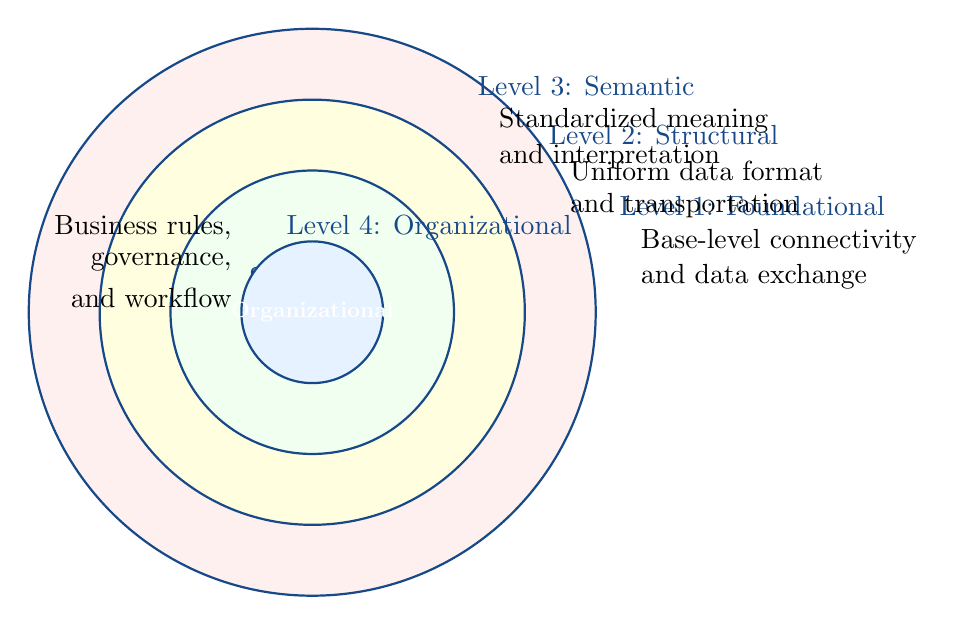
\begin{tikzpicture}[scale=0.9]
            % Four levels as concentric rings
            \draw[fill=lightred, draw=darkblue, thick] (0,0) circle (4cm);
            \node[darkblue, font=\bfseries] at (0,0) {Foundational};
            
            \draw[fill=lightyellow, draw=darkblue, thick] (0,0) circle (3cm);
            \node[darkblue, font=\bfseries] at (0,0.5) {Structural};
            
            \draw[fill=lightgreen, draw=darkblue, thick] (0,0) circle (2cm);
            \node[darkblue, font=\bfseries] at (0,0.5) {Semantic};
            
            \draw[fill=lightblue, draw=darkblue, thick] (0,0) circle (1cm);
            \node[white, font=\bfseries, scale=0.8] at (0,0) {Organizational};
            
            % Labels around the rings
            \node[darkblue, anchor=west] at (4.2,1.5) {Level 1: Foundational};
            \node[anchor=west] at (4.5,1) {Base-level connectivity};
            \node[anchor=west] at (4.5,0.5) {and data exchange};
            
            \node[darkblue, anchor=west] at (3.2,2.5) {Level 2: Structural};
            \node[anchor=west] at (3.5,2) {Uniform data format};
            \node[anchor=west] at (3.5,1.5) {and transportation};
            
            \node[darkblue, anchor=west] at (2.2,3.2) {Level 3: Semantic};
            \node[anchor=west] at (2.5,2.7) {Standardized meaning};
            \node[anchor=west] at (2.5,2.2) {and interpretation};
            
            \node[darkblue, anchor=west] at (-0.5,1.2) {Level 4: Organizational};
            \node[anchor=east] at (-1,1.2) {Business rules,};
            \node[anchor=east] at (-1,0.7) {governance,};
            \node[anchor=east] at (-1,0.2) {and workflow};
        \end{tikzpicture}
    \end{center}
    
    \smallskip
    
    The Healthcare Information and Management Systems Society (HIMSS) framework distinguishes four levels of interoperability, each building upon the previous to enable progressively more sophisticated information exchange and cooperative use \cite{HIMSS2019}.
\end{frame}

\begin{frame}{Level 1: Foundational Interoperability}
    \begin{columns}
        \begin{column}{0.5\textwidth}
            \begin{block}{Definition}
                Foundational interoperability enables one information system to receive data from another and store it appropriately. It establishes the basic technical capability for systems to connect and exchange data without requiring the receiving system to interpret the data's meaning.
            \end{block}
        \end{column}
        \begin{column}{0.5\textwidth}
            \begin{block}{Technical Requirements}
                \begin{itemize}
                    \item Network connectivity and communication protocols
                    \item Interface APIs and data transmission methods
                    \item Basic security and authentication
                    \item File transfer and message transport capabilities
                    \item Hardware and infrastructure compatibility
                \end{itemize}
            \end{block}
        \end{column}
    \end{columns}
    
    \pause
    
    \begin{block}{Current Status}
        Most modern health information systems achieve foundational interoperability through web services, REST APIs, and standard transport protocols. However, this technical capability does not ensure that exchanged data can be understood or used effectively by receiving systems.
    \end{block}
\end{frame}

\begin{frame}{Level 2: Structural Interoperability}
    \begin{columns}
        \begin{column}{0.5\textwidth}
            \begin{block}{Definition}
                Structural interoperability defines the format, syntax, and organization of data exchange. It ensures that data transmitted between systems can be parsed and displayed in a way that preserves the clinical meaning and structure of the original information.
            \end{block}
        \end{column}
        \begin{column}{0.5\textwidth}
            \begin{block}{Syntactic Standards}
                \begin{itemize}
                    \item HL7 v2.x message structures
                    \item HL7 CDA document standards
                    \item XML and JSON data formats
                    \item DICOM for medical imaging
                    \item IHE transaction profiles
                \end{itemize}
            \end{block}
        \end{column}
    \end{columns}
    
    \pause
    
    \begin{block}{The Structure-Content Distinction}
        While structural interoperability ensures that data elements arrive in the correct format with proper organization, it does not address whether the receiving system assigns the same meaning to those elements. Two systems may successfully exchange data while interpreting it differently.
    \end{block}
\end{frame}

\begin{frame}{Level 3: Semantic Interoperability}
    \begin{center}
        \begin{tikzpicture}[scale=0.85]
            % Semantic interoperability diagram
            \draw[fill=lightblue, draw=darkblue, thick] (0,0) rectangle (12,6);
            
            \node[darkblue, font=\bfseries, fontsize=14] at (6,5.3) {Semantic Interoperability};
            
            % Left system
            \draw[fill=darkblue, draw=none] (1,1) rectangle (4,4);
            \node[white, font=\small] at (2.5,2.5) {System A};
            \node[white, font=\small, scale=0.8] at (2.5,1.5) {Diagnosis:};
            \node[white, font=\small, scale=0.8] at (2.5,1.2) {``Type 2 Diabetes''};
            
            % Center - terminology translation
            \draw[fill=accent, draw=darkblue, thick] (4.5,2) rectangle (7.5,4);
            \node[white, font=\small] at (6,3) {Terminology};
            \node[white, font=\small] at (6,2.6) {Service};
            \node[white, font=\small] at (6,2.2) {(FHIR CodeSystem)};
            
            % Arrow with terminology mapping
            \draw[<->, thick] (4,2.5) -- (4.5,2.5);
            \draw[<->, thick] (7.5,2.5) -- (8,2.5);
            
            % Right system
            \draw[fill=darkblue, draw=none] (8,1) rectangle (11,4);
            \node[white, font=\small] at (9.5,2.5) {System B};
            \node[white, font=\small, scale=0.8] at (9.5,1.5) {Diagnosis:};
            \node[white, font=\small, scale=0.8] at (9.5,1.2) {E11.9 (ICD-10)};
            
            % Concept representation
            \node[darkblue, font=\small, anchor=center] at (6,1) {SNOMED CT: 44054006 | ICD-10: E11.9 | LOINC: 85318-4};
        \end{tikzpicture}
    \end{center}
    
    \smallskip
    
    Semantic interoperability represents the highest level of data exchange, where systems share a common understanding of data meaning. This requires standardized terminologies, ontologies, and mapping services that translate between different coding systems while preserving clinical significance \cite{McDonald2015}.
\end{frame}

\begin{frame}{Level 4: Organizational Interoperability}
    \begin{columns}
        \begin{column}{0.5\textwidth}
            \begin{block}{Definition}
                Organizational interoperability encompasses the social, legal, organizational, and governance dimensions that enable seamless information exchange across institutional boundaries. It addresses the business rules, workflows, and trust relationships necessary for effective cooperation.
            \end{block}
        \end{column}
        \begin{column}{0.5\textwidth}
            \begin{block}{Organizational Elements}
                \begin{itemize}
                    \item Governance frameworks and data sharing agreements
                    \item Consent management and patient authorization
                    \item Trust frameworks and credentialing
                    \item Business process alignment
                    \item Liability and accountability assignment
                    \item Sustainability and funding models
                \end{itemize}
            \end{block}
        \end{column}
    \end{columns}
    
    \pause
    
    \begin{block}{The Ultimate Challenge}
        Organizational interoperability is often the most difficult to achieve, requiring coordination across multiple stakeholders with different interests, cultures, and legal frameworks. Without organizational alignment, technical and semantic interoperability alone are insufficient for effective health information exchange \cite{Jensen2019}.
    \end{block}
\end{frame}

%=======================================================================
% SECTION 3: INTERNATIONAL STANDARDS LANDSCAPE
%=======================================================================
\section{International Standards Landscape}

\begin{frame}{Health Standards Organizations}
    \begin{center}
        \begin{tabular}{@{}lp{6cm}@{}}
            \toprule
            \textbf{Organization} & \textbf{Key Standards and Role} \\
            \midrule
            \textbf{HL7 International} & Clinical document standards, messaging protocols, FHIR specification \\
            \textbf{IHTSDO (SNOMED International)} & Clinical terminology and ontology standards \\
            \textbf{WHO (FIC)} & ICD classification, international health terminology governance \\
            \textbf{IHE International} & Integration profiles and implementation frameworks \\
            \textbf{ISO TC 215} & Health informatics standards development \\
            \textbf{DICOM Standards} & Medical imaging storage and transmission \\
            \textbf{LOINC} & Laboratory and clinical observation standards \\
            \bottomrule
        \end{tabular}
    \end{center}
    
    \pause
    
    \begin{block}{The Standards Ecosystem}
        Multiple international bodies develop health informatics standards, creating a complex landscape that requires coordination and alignment. While this diversity reflects the breadth of health information challenges, it also creates integration challenges for implementers \cite{benson2019}.
    \end{block}
\end{frame}

\begin{frame}{HL7 and FHIR: The Current Standard}
    \begin{columns}
        \begin{column}{0.5\textwidth}
            \begin{block}{HL7 v2.x Legacy}
                \begin{itemize}
                    \item Developed in the 1980s-1990s
                    \item Message-based text protocol
                    \item Widely implemented globally
                    \item Flexible but inconsistently used
                    \item Being phased out in favor of newer standards
                    \item Still dominant in LMIC settings
                \end{itemize}
            \end{block}
        \end{column}
        \begin{column}{0.5\textwidth}
            \begin{block}{HL7 FHIR (Fast Healthcare Interoperability Resources)}
                \begin{itemize}
                    \item Modern web standards (REST, JSON, XML)
                    \item Designed for contemporary app development
                    \item Human-readable and machine-parseable
                    \item Growing implementation globally
                    \item US Core data elements and SMART on FHIR
                    \item Preferred standard for new implementations
                \end{itemize}
            \end{block}
        \end{column}
    \end{columns}
    
    \pause
    
    \begin{block}{FHIR Adoption Trajectory}
        FHIR has emerged as the dominant standard for new health information exchange, supported by major EHR vendors and governments. However, the installed base of HL7 v2.x systems means most real-world exchange still involves legacy protocols and associated translation challenges \cite{bloom2019}.
    \end{block}
\end{frame}

\begin{frame}{Clinical Terminology Standards}
    \begin{center}
        \begin{tabular}{@{}lp{6cm}@{}}
            \toprule
            \textbf{Standard} & \textbf{Application and Coverage} \\
            \midrule
            \textbf{ICD-10/ICD-11} & Disease classification for mortality, morbidity, billing \\
            \textbf{SNOMED CT} & Comprehensive clinical terminology for documentation \\
            \textbf{LOINC} & Laboratory tests, clinical observations, survey instruments \\
            \textbf{RxNorm} & Normalized names for clinical drugs and combinations \\
            \textbf{CPT/HCPCS} & Procedures and services for billing (US-specific) \\
            \textbf{ATC} & Anatomical Therapeutic Chemical drug classification \\
            \bottomrule
        \end{tabular}
    \end{center}
    
    \pause
    
    \begin{block}{The Mapping Challenge}
        Different terminologies serve different purposes and contexts. Implementing semantic interoperability requires understanding the relationships between these standards, establishing cross-maps, and managing the inevitable information loss that occurs when translating between systems with different granularity and scope \cite{richards2018}.
    \end{block}
\end{frame}

\begin{frame}{IHE Integration Profiles}
    \begin{columns}
        \begin{column}{0.5\textwidth}
            \begin{block}{What are IHE Profiles?}
                The Integrating the Healthcare Enterprise (IHE) initiative develops implementation guides that specify how standards should be used to address specific integration scenarios. These profiles define the actors, transactions, and workflows necessary for effective information exchange.
            \end{block}
        \end{column}
        \begin{column}{0.5\textwidth}
            \begin{block}{Key IHE Domains}
                \begin{itemize}
                    \item \textbf{Cardiology}: Echocardiography, ECG exchange
                    \item \textbf{Radiology}: Imaging document sharing, query-retrieve
                    \item \textbf{Laboratory}: Lab reporting, result delivery
                    \item \textbf{Patient Care Coordination}: Care management, referral workflows
                    \item \textbf{Patient Administration}: Admission, discharge, transfer
                \end{itemize}
            \end{block}
        \end{column}
    \end{columns}
    
    \pause
    
    \begin{block}{IHE Value Proposition}
        IHE profiles reduce the specification burden on implementers by providing tested, consensus-based integration patterns. When vendors claim IHE compliance, purchasers have confidence that their systems will work with other IHE-compliant systems for specified use cases \cite{IHE2020}.
    \end{block}
\end{frame}

%=======================================================================
% SECTION 4: CHALLENGES - FRAGMENTED SYSTEMS
%=======================================================================
\section{Challenge 1: Fragmented Systems and Legacy Platforms}

\begin{frame}{The Legacy System Burden}
    \begin{columns}
        \begin{column}{0.5\textwidth}
            \begin{block}{Legacy System Characteristics}
                \begin{itemize}
                    \item Proprietary data formats and structures
                    \item Outdated programming languages and architectures
                    \item Limited or no interface capabilities
                    \item High maintenance costs
                    \item Vendor no longer in business
                    \item Institutional dependency and embedded workflows
                \end{itemize}
            \end{block}
        \end{column}
        \begin{column}{0.5\textwidth}
            \begin{block}{The Sunk Cost Dilemma}
                \begin{itemize}
                    \item Organizations have invested millions in current systems
                    \item Staff have learned to work around limitations
                    \item Data accumulated over decades is trapped
                    \item Disruption to clinical workflows during migration
                    \item Uncertainty about new system capabilities
                    \item Vendor lock-in through contracts and customization
                \end{itemize}
            \end{block}
        \end{column}
    \end{columns}
    
    \pause
    
    \begin{block}{The Migration Challenge}
        Replacing legacy systems is rarely feasible due to data migration complexity, workflow disruption, and cost. More commonly, organizations implement interface engines and middleware to bridge legacy systems with newer standards, creating layered architectures that add complexity and maintenance burden \cite{lahyani2019}.
    \end{block}
\end{frame}

\begin{frame}{Vertical Program Fragmentation}
    \begin{center}
        \begin{tikzpicture}[scale=0.9]
            % Fragmented system visualization
            \draw[fill=lightblue, draw=darkblue, thick] (0,0) rectangle (12,7);
            
            \node[darkblue, font=\bfseries, fontsize=14] at (6,6.3) {Vertical Program Fragmentation in LMICs};
            
            % Vertical silos
            \draw[fill=darkblue, draw=none] (1,1) rectangle (3,5);
            \node[white, font=\small] at (2,3) {HIV/AIDS\\Program};
            
            \draw[fill=accent, draw=none] (3.5,1) rectangle (5.5,5);
            \node[white, font=\small] at (4.5,3) {TB Program};
            
            \draw[fill=orange, draw=none] (6,1) rectangle (8,5);
            \node[white, font=\small] at (7,3) {Malaria\\Program};
            
            \draw[fill=green!70, draw=none] (8.5,1) rectangle (10.5,5);
            \node[white, font=\small] at (9.5,3) {Maternal\\Health};
            
            % Vertical arrows
            \draw[<->, thick, red] (3,2) -- (3.5,2);
            \draw[<->, thick, red] (5.5,3) -- (6,3);
            \draw[<->, thick, red] (8,4) -- (8.5,4);
            
            % No horizontal integration
            \node[red, font=\small] at (4.75,1.2) {No data exchange};
            \node[red, font=\small] at (7.25,1.2) {No data exchange};
            
            % Bottom layer - patient
            \draw[fill=darkblue, draw=none] (3,0.3) rectangle (9,0.7);
            \node[white, font=\small] at (6,0.5) {The Patient};
            
            % Patient arrows to each silo
            \foreach \x in {2,4.5,7,9.5} {
                \draw[->, thick, accent] (6,0.3) -- (\x,1);
            }
        \end{tikzpicture}
    \end{center}
    
    \smallskip
    
    In many LMICs, donor-funded vertical disease programs implement parallel information systems that cannot communicate with each other or with national health information systems, creating a fragmented landscape where patients may be represented in multiple systems without any system having a complete picture \cite{braa2012}.
\end{frame}

\begin{frame}{Case Study: India's Digital Health Ecosystem}
    \begin{columns}
        \begin{column}{0.5\textwidth}
            \begin{block}{Current Complexity}
                \begin{itemize}
                    \item Multiple state-level EMR systems with no national standardization
                    \item Private sector using diverse commercial products
                    \item National programs (NPCDCS, NLEP, RNTCP) with separate reporting
                    \item Insurance schemes (Ayushman Bharat, state schemes) with separate databases
                    \item Labs and pharmacies operating independent systems
                \end{itemize}
            \end{block}
        \end{column}
        \begin{column}{0.5\textwidth}
            \begin{block}{Government Response}
                \begin{itemize}
                    \item Ayushman Bharat Digital Mission (ABDM) establishing national architecture
                    \item Unique Health ID for every citizen
                    \item Health Information Exchange and Consent Manager (HIE-CM)
                    \item Personal Health Record (PHR) framework
                    \item Mandatory FHIR-based data exchange for public facilities
                \end{itemize}
            \end{block}
        \end{column}
    \end{columns}
    
    \pause
    
    \begin{block}{Implementation Challenges}
        Despite ambitious policy, India's digital health transformation faces challenges in legacy system migration, private sector participation incentives, digital literacy gaps, and the sheer scale of implementing standardization across thousands of independent facilities \cite{joshi2020}.
    \end{block}
\end{frame}

%=======================================================================
% SECTION 5: CHALLENGES - STANDARDS ADOPTION
%=======================================================================
\section{Challenge 2: Standards Adoption and Implementation Gaps}

\begin{frame}{The Standards Adoption Gap}
    \begin{center}
        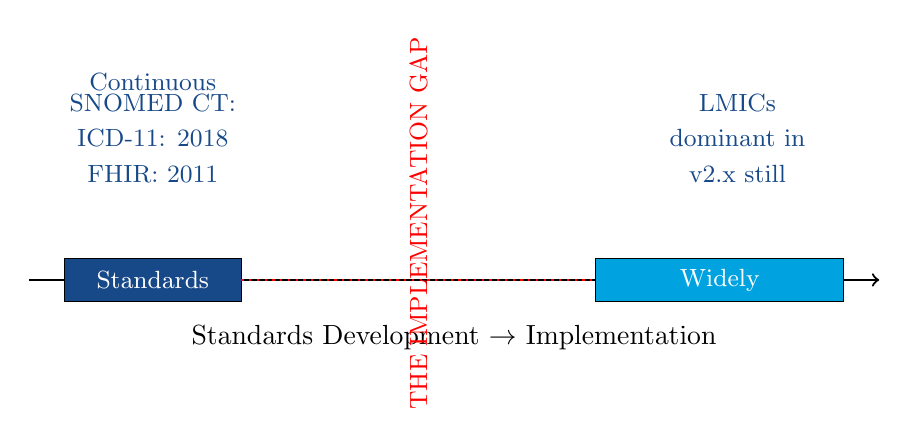
\begin{tikzpicture}[scale=0.9]
            % Gap visualization
            \draw[->, thick] (0,0) -- (12,0);
            \node[anchor=north] at (6,-0.5) {Standards Development $\rightarrow$ Implementation};
            
            % Standards development
            \draw[fill=darkblue] (0.5,-0.3) rectangle (3,0.3);
            \node[white, font=\small] at (1.75,0) {Standards};
            \node[white, font=\small] at (1.75,-0.5) {Developed};
            
            % Gap
            \draw[dotted, thick, red] (3,0) -- (8,0);
            \node[red, font=\small, rotate=90] at (5.5,0.8) {THE IMPLEMENTATION GAP};
            
            % Implementation
            \draw[fill=accent] (8,-0.3) rectangle (11.5,0.3);
            \node[white, font=\small] at (9.75,0) {Widely};
            \node[white, font=\small] at (9.75,-0.5) {Implemented};
            
            % Timeline indicators
            \node[darkblue, font=\small] at (1.75,1.5) {FHIR: 2011};
            \node[darkblue, font=\small] at (1.75,2) {ICD-11: 2018};
            \node[darkblue, font=\small] at (1.75,2.5) {SNOMED CT:};
            \node[darkblue, font=\small] at (1.75,2.8) {Continuous};
            
            \node[darkblue, font=\small] at (10,1.5) {v2.x still};
            \node[darkblue, font=\small] at (10,2) {dominant in};
            \node[darkblue, font=\small] at (10,2.5) {LMICs};
        \end{tikzpicture}
    \end{center}
    
    \smallskip
    
    A significant gap exists between standards development and actual implementation. While sophisticated international standards exist, practical adoption is limited by lack of awareness, implementation complexity, resource constraints, and insufficient technical support capacity \cite{lehne2019}.
\end{frame}

\begin{frame}{Implementation Barriers}
    \begin{columns}
        \begin{column}{0.5\textwidth}
            \begin{block}{Technical Barriers}
                \begin{itemize}
                    \item Standards complexity and documentation quality
                    \item Multiple conflicting implementation guides
                    \item Insufficient test infrastructure and tools
                    \item Limited testing and conformance certification
                    \item Integration with legacy systems
                    \item Performance and scalability concerns
                \end{itemize}
            \end{block}
        \end{column}
        \begin{column}{0.5\textwidth}
            \begin{block}{Non-Technical Barriers}
                \begin{itemize}
                    \item Competing vendor interests and business models
                    \item Insufficient human capacity and training
                    \item Weak regulatory requirements and incentives
                    \item Fragmented stakeholder coordination
                    \item Cost of implementation and certification
                    \item Lack of proven business case
                \end{itemize}
            \end{block}
        \end{column}
    \end{columns}
    
    \pause
    
    \begin{block}{The Certification Void}
        Unlike other industries (telecommunications, financial services), health informatics lacks universal certification requirements. Vendors can claim standards compliance without verification, creating uncertainty for purchasers and limiting confidence in actual interoperability capabilities \cite{RHIA2018}.
    \end{block}
\end{frame}

\begin{frame}{The Conformance Challenge}
    \begin{columns}
        \begin{column}{0.5\textwidth}
            \begin{block}{Levels of Conformance}
                \begin{itemize}
                    \item \textbf{No conformance}: Systems using proprietary formats
                    \item \textbf{Document-level}: Exporting standards-compliant documents but no structured data
                    \item \textbf{Element-level}: Exchanging structured data elements but inconsistent semantics
                    \item \textbf{Full conformance}: Complete, standards-compliant exchange with semantic alignment
                \end{itemize}
            \end{block}
        \end{column}
        \begin{column}{0.5\textwidth}
            \begin{block}{The Reality Gap}
                Most systems claiming HL7 or FHIR implementation actually support only partial conformance. A study of US hospitals found that while 96\% reported having certified EHR technology, only 38\% could successfully exchange data with external organizations using standardized methods.
            \end{block}
        \end{column}
    \end{columns}
    
    \pause
    
    \begin{block}{The Interoperability Paradox}
        Organizations may claim full interoperability while actually supporting only basic data exchange. Without rigorous testing and certification, claims of standards compliance provide limited assurance of actual exchange capability, undermining trust and adoption \cite{Adashi2018}.
    \end{block}
\end{frame}

%=======================================================================
% SECTION 6: CHALLENGES - GOVERNANCE AND POLICY
%=======================================================================
\section{Challenge 3: Governance, Policy, and Regulatory Issues}

\begin{frame}{Governance Fragmentation}
    \begin{columns}
        \begin{column}{0.5\textwidth}
            \begin{block}{Multi-Level Governance Challenges}
                \begin{itemize}
                    \item Multiple government ministries with overlapping authority (health, ICT, privacy)
                    \item National versus sub-national (state, provincial) jurisdiction conflicts
                    \item Public versus private sector regulatory differences
                    \item International data flow and sovereignty issues
                    \item Professional licensing and scope of practice regulations
                \end{itemize}
            \end{block}
        \end{column}
        \begin{column}{0.5\textwidth}
            \begin{block}{Stakeholder Misalignment}
                \begin{itemize}
                    \item Vendors prioritize features that drive sales over interoperability
                    \item Providers resist mandates perceived as unfunded mandates
                    \item Patients lack voice in data governance decisions
                    \item Regulators struggle to keep pace with technology evolution
                    \item Donors prioritize short-term program goals over systemic interoperability
                \end{itemize}
            \end{block}
        \end{column}
    \end{columns}
    
    \pause
    
    \begin{block}{The Coordination Imperative}
        Effective health information governance requires coordination across multiple stakeholders with different authorities, interests, and capacities. Weak governance coordination leads to policy fragmentation, conflicting requirements, and implementation chaos at the operational level \cite{scott2018}.
    \end{block}
\end{frame}

\begin{frame}{Policy and Regulatory Gaps}
    \begin{center}
        \begin{tabular}{@{}lp{6cm}@{}}
            \toprule
            \textbf{Policy Area} & \textbf{Common Gaps} \\
            \midrule
            \textbf{Mandates and Incentives} & Voluntary participation without accountability or reward \\
            \textbf{Privacy and Consent} & Weak legal frameworks, inconsistent enforcement \\
            \textbf{Data Ownership} & Unclear rights and responsibilities for health data \\
            \textbf{Interoperability Requirements} & No mandatory standards, vague compliance definitions \\
            \textbf{Data Quality} & No requirements for accuracy, completeness, timeliness \\
            \textbf{Penalties} & No consequences for non-compliance or data breaches \\
            \bottomrule
        \end{tabular}
    \end{center}
    
    \pause
    
    \begin{block}{The Regulatory Void}
        Many jurisdictions lack comprehensive health informatics legislation, leaving interoperability to market forces and voluntary initiatives. Without clear policy direction, stakeholders lack the certainty needed to make long-term investments in standards-based systems \cite{abbas2019}.
    \end{block}
\end{frame}

\begin{frame}{Case Study: European Health Data Space}
    \begin{columns}
        \begin{column}{0.5\textwidth}
            \begin{block}{Policy Framework}
                \begin{itemize}
                    \item Regulation establishing common European health data space
                    \item Mandatory FHIR-based exchange for cross-border care
                    \item Strong data protection requirements (GDPR)
                    \item Secondary use provisions for research and policy
                    \item Infrastructure for cross-border authentication
                    \item Governance structures at EU and member state levels
                \end{itemize}
            \end{block}
        \end{column}
        \begin{column}{0.5\textwidth}
            \begin{block}{Challenges and Lessons}
                \begin{itemize}
                    \item Balancing harmonization with member state autonomy
                    \item Technical complexity of cross-border exchange
                    \item Varying digital maturity across member states
                    \item Privacy concerns and public trust
                    \item Funding and sustainability questions
                    \item Timeline for full implementation (estimated 2025+)
                \end{itemize}
            \end{block}
        \end{column}
    \end{columns}
    
    \pause
    
    \begin{block}{Relevance for Other Regions}
        The European Health Data Space represents the most ambitious attempt at regional health data integration, providing lessons in governance structure, technical architecture, and the political economy of multi-country coordination. However, its complexity and cost illustrate the challenges of similar efforts elsewhere \cite{EuropeanCommission2021}.
    \end{block}
\end{frame}

%=======================================================================
% SECTION 7: CHALLENGES - DATA QUALITY AND PRIVACY
%=======================================================================
\section{Challenge 4: Data Quality, Privacy, and Security Concerns}

\begin{frame}{Data Quality as Interoperability Foundation}
    \begin{columns}
        \begin{column}{0.5\textwidth}
            \begin{block}{Data Quality Dimensions}
                \begin{itemize}
                    \item \textbf{Accuracy}: Data correctly represents the real-world entity
                    \item \textbf{Completeness}: Required data elements are present
                    \item \textbf{Timeliness}: Data is current and updated appropriately
                    \item \textbf{Consistency}: Data is coherent across sources and over time
                    \item \textbf{Validity}: Data conforms to defined rules and formats
                \end{itemize}
            \end{block}
        \end{column}
        \begin{column}{0.5\textwidth}
            \begin{block}{Quality in Exchange Context}
                \begin{itemize}
                    \item Poor quality data exported becomes poor quality data everywhere
                    \item Lack of data provenance tracking
                    \item Missing contextual information limiting interpretation
                    \item Duplicate records and patient matching failures
                    \item Terminology variation and mapping errors
                    \item Inconsistent documentation practices
                \end{itemize}
            \end{block}
        \end{column}
    \end{columns}
    
    \pause
    
    \begin{block}{Garbage In, Garbage Out}
        Interoperability systems can efficiently exchange data, but they cannot create quality from poor source data. Investment in data quality at the point of capture is prerequisite to meaningful interoperability at the exchange level \cite{kahn2019}.
    \end{block}
\end{frame}

\begin{frame}{Patient Matching and Identity Management}
    \begin{center}
        \begin{tikzpicture}[scale=0.85]
            % Patient matching problem
            \draw[fill=lightblue, draw=darkblue, thick] (0,0) rectangle (12,6);
            
            \node[darkblue, font=\bfseries, fontsize=14] at (6,5.3) {The Patient Matching Challenge};
            
            % Multiple representations
            \draw[fill=darkblue, draw=none] (1,1) rectangle (4,4);
            \node[white, font=\small] at (2.5,2.8) {Hospital A};
            \node[white, font=\small, scale=0.8] at (2.5,2.2) {John Smith};
            \node[white, font=\small, scale=0.8] at (2.5,1.8) {DOB: 03/15/1975};
            \node[white, font=\small, scale=0.8] at (2.5,1.4) {ID: 12345};
            
            \draw[fill=accent, draw=none] (4.5,1) rectangle (7.5,4);
            \node[white, font=\small] at (6,2.8) {Clinic B};
            \node[white, font=\small, scale=0.8] at (6,2.2) {Jonathon Smith};
            \node[white, font=\small, scale=0.8] at (6,1.8) {DOB: 03/15/1975};
            \node[white, font=\small, scale=0.8] at (6,1.4) {MRN: 98765};
            
            \draw[fill=orange, draw=none] (8,1) rectangle (11,4);
            \node[white, font=\small] at (9.5,2.8) {Pharmacy C};
            \node[white, font=\small, scale=0.8] at (9.5,2.2) {J. Smith};
            \node[white, font=\small, scale=0.8] at (9.5,1.8) {DOB: 03/15/75};
            \node[white, font=\small, scale=0.8] at (9.5,1.4) {Rx: 11111};
            
            % Question mark
            \node[red, font=\Large] at (6,0.5) {Same patient? Different patients?};
            
            % Statistics
            \node[darkblue, font=\small, anchor=west] at (0.5,5.5) {Studies suggest 8-12\% of patient records are duplicates};
        \end{tikzpicture}
    \end{center}
    
    \smallskip
    
    Without reliable patient matching, information exchanged may be attributed to the wrong individual, creating safety risks and undermining clinical utility. Unique patient identifiers, deterministic and probabilistic matching algorithms, and governance frameworks are all required to address this challenge \cite{Grannis2019}.
\end{frame}

\begin{frame}{Privacy, Security, and Trust}
    \begin{columns}
        \begin{column}{0.5\textwidth}
            \begin{block}{Security Concerns}
                \begin{itemize}
                    \item Increased attack surface with more connected systems
                    \item Healthcare second only to financial sector in breach incidents
                    \item Ransomware attacks on hospitals disrupting care delivery
                    \item Insider threats from authorized users
                    \item Legacy systems with outdated security
                    \item IoT medical devices with limited security
                \end{itemize}
            \end{block}
        \end{column}
        \begin{column}{0.5\textwidth}
            \begin{block}{Privacy Considerations}
                \begin{itemize}
                    \item Sensitive health data requires strong protections
                    \item Consent management across multiple use cases
                    \item Secondary use of clinical data for research
                    \item Data retention and deletion requirements
                    \item Cross-border data flow restrictions
                    \item Right to access and correct personal data
                \end{itemize}
            \end{block}
        \end{column}
    \end{columns}
    
    \pause
    
    \begin{block}{The Trust Imperative}
        Patients and providers must trust that shared data will be protected and used appropriately. High-profile breaches and misuse incidents erode trust, reducing willingness to participate in information exchange and undermining the interoperability infrastructure \cite{cohen2018}.
    \end{block}
\end{frame}

%=======================================================================
% SECTION 8: CHALLENGES - HUMAN CAPACITY
%=======================================================================
\section{Challenge 5: Human Capacity and Organizational Barriers}

\begin{frame}{The Health Informatics Skills Gap}
    \begin{columns}
        \begin{column}{0.5\textwidth}
            \begin{block}{Capacity Shortages}
                \begin{itemize}
                    \item Global shortage of health informatics professionals
                    \item Inadequate training programs in LMICs
                    \item Limited exposure during health professional education
                    \item Rapid technology evolution outpacing skill development
                    \item Brain drain to private sector and high-income countries
                    \item Weak career pathways and recognition
                \end{itemize}
            \end{block}
        \end{column}
        \begin{column}{0.5\textwidth}
            \begin{block}{Skills Required}
                \begin{itemize}
                    \item Clinical informatics understanding
                    \item Health data standards knowledge
                    \item Software development and systems integration
                    \item Project management and change leadership
                    \item Data analysis and interpretation
                    \item Communication across technical and clinical domains
                \end{itemize}
            \end{block}
        \end{column}
    \end{columns}
    
    \pause
    
    \begin{block}{The Bridge Role Gap}
        Organizations struggle to find professionals who can bridge clinical, technical, and leadership domains. This ``T-shaped'' skill profile—deep expertise in one area with broad understanding of related fields—is rare and increasingly in demand \cite{saeed2019}.
    \end{block}
\end{frame}

\begin{frame}{Organizational and Cultural Barriers}
    \begin{center}
        \begin{tabular}{@{}lp{6cm}@{}}
            \toprule
            \textbf{Barrier Type} & \textbf{Impact on Interoperability} \\
            \midrule
            \textbf{Organizational silos} & Departments protect data as organizational asset \\
            \textbf{Culture of autonomy} & Reluctance to share data with external entities \\
            \textbf{Change resistance} & Staff prefer existing workflows over new systems \\
            \textbf{Lack of leadership} & No executive sponsorship for interoperability initiatives \\
            \textbf{Weak governance} & No accountability for data quality and exchange \\
            \textbf{Business model conflicts} & Vendor lock-in as competitive advantage \\
            \bottomrule
        \end{tabular}
    \end{center}
    
    \pause
    
    \begin{block}{The People Problem}
        Technical solutions cannot overcome organizational and cultural barriers to interoperability. Leadership commitment, change management, governance frameworks, and aligned incentives are prerequisites for successful implementation of any interoperability infrastructure \cite{peterson2019}.
    \end{block}
\end{frame}

%=======================================================================
% SECTION 9: LMIC CASE STUDIES
%=======================================================================
\section{Case Studies: LMIC Health System Examples}

\begin{frame}{Case Study: Rwanda's Health Information Revolution}
    \begin{columns}
        \begin{column}{0.5\textwidth}
            \begin{block}{Achievements}
                \begin{itemize}
                    \item National rollout of DHIS2 to all 500+ health facilities
                    \item RapidSMS for community health worker reporting
                    \item Electronic Medical Record system in referral hospitals
                    \item Integration of vertical programs into national HIS
                    \item Mobile health coverage reaching 95\% of population
                \end{itemize}
            \end{block}
        \end{column}
        \begin{column}{0.5\textwidth}
            \begin{block}{Key Success Factors}
                \begin{itemize}
                    \item Strong government ownership and leadership
                    \item Integration with community health worker programs
                    \item Phased implementation with continuous learning
                    \item Investment in human capacity at all levels
                    \item Partnerships with academic and international partners
                    \item Leveraging mobile infrastructure for last-mile reach
                \end{itemize}
            \end{block}
        \end{column}
    \end{columns}
    
    \pause
    
    \begin{block}{Lessons Learned}
        Rwanda demonstrates that LMICs can achieve meaningful health information system integration with appropriate leadership, partnerships, and incremental capacity building. However, challenges remain in achieving full semantic interoperability and integrating private sector data \cite{nyirabagabo2020}.
    \end{block}
\end{frame}

\begin{frame}{Case Study: Brazil's SUS Information System}
    \begin{columns}
        \begin{column}{0.5\textwidth}
            \begin{block}{Scale and Complexity}
                \begin{itemize}
                    \item World's largest public health system (220+ million users)
                    \item Decentralized governance across 5,500+ municipalities
                    \item Family Health Strategy covering 65\% of population
                    \item Mix of federal, state, and municipal systems
                    \item Significant private sector parallel system
                \end{itemize}
            \end{block}
        \end{column}
        \begin{column}{0.5\textwidth}
            \begin{block}{Interoperability Challenges}
                \begin{itemize}
                    \item Historical fragmentation across political periods
                    \item Limited federal leverage over municipal autonomy
                    \item Commercial vendor dominance in municipal systems
                    \item Data quality and completeness inconsistencies
                    \item Citizen ID not linked to health records
                    \item Gradual progress toward e-SUS AB standardization
                \end{itemize}
            \end{block}
        \end{column}
    \end{columns}
    
    \pause
    
    \begin{block}{The Decentralization Challenge}
        Brazil illustrates the interoperability challenges of highly decentralized health systems where municipal autonomy limits standardization efforts. Progress requires balancing local flexibility with national coordination, often through incentive structures rather than mandates \cite{mendes2019}.
    \end{block}
\end{frame}

\begin{frame}{Case Study: Kenya's Digital Health Landscape}
    \begin{columns}
        \begin{column}{0.5\textwidth}
            \begin{block}{Current State}
                \begin{itemize}
                    \item KHIS (Kenya Health Information System) built on DHIS2
                    \item Multiple program-specific systems (HIV, TB, malaria)
                    \item mHealth initiatives including SMS-based programs
                    \item Afya Nyumbani Duval winde 2.0 for facility reporting
                    \item Emerging discussions on national EMR strategy
                \end{itemize}
            \end{block}
        \end{column}
        \begin{column}{0.5\textwidth}
            \begin{block}{Interoperability Priorities}
                \begin{itemize}
                    \item Harmonizing donor-funded vertical systems
                    \item Establishing national health information exchange
                    \item Developing master facility registry
                    \item Implementing unique patient identifiers
                    \item Building standards-based exchange infrastructure
                    \item Addressing human capacity gaps
                \end{itemize}
            \end{block}
        \end{column}
    \end{columns}
    
    \pause
    
    \begin{block}{The Donor Coordination Challenge}
        Kenya's experience illustrates the complexity of coordinating multiple donor-funded health programs, each with its own information system requirements. The government's emerging digital health strategy aims to establish governance structures that align donor priorities with national interoperability goals \cite{wasunna2020}.
    \end{block}
\end{frame}

%=======================================================================
% SECTION 10: IMPLICATIONS FOR HEALTH SYSTEM PERFORMANCE
%=======================================================================
\section{Implications for Health System Performance}

\begin{frame}{Impact on Care Continuity}
    \begin{center}
        \begin{tabular}{@{}lp{6cm}@{}}
            \toprule
            \textbf{Interoperability Gap} & \textbf{Impact on Care Continuity} \\
            \midrule
            \textbf{Patient record fragmentation} & Incomplete information at point of care; repeat testing \\
            \textbf{Referral information loss} & Delayed or ineffective care transitions \\
            \textbf{Medication reconciliation failures} & Adverse drug events, duplicative therapy \\
            \textbf{Lab and imaging siloing} & Delayed diagnosis; conflicting results \\
            \textbf{Provider communication gaps} & Care plan misalignment; duplicated efforts \\
            \bottomrule
        \end{tabular}
    \end{center}
    
    \pause
    
    \begin{block}{The Continuity Cost}
        Lack of interoperability undermines the fundamental requirement for continuity of information across care episodes and providers. Patients experience fragmented care, providers make decisions with incomplete information, and health systems bear unnecessary costs from duplicated services and preventable adverse events \cite{van Allen2018}.
    \end{block}
\end{frame}

\begin{frame}{Impact on Health System Efficiency}
    \begin{columns}
        \begin{column}{0.5\textwidth}
            \begin{block}{Resource Wastage}
                \begin{itemize}
                    \item Duplicate testing due to unavailable prior results
                    \item Time spent searching for and reconciling data
                    \item Manual data entry and transcription errors
                    \item Workflow interruptions from system incompatibility
                    \item Inefficient care coordination across settings
                \end{itemize}
            \end{block}
        \end{column}
        \begin{column}{0.5\textwidth}
            \begin{block}{Lost Opportunities}
                \begin{itemize}
                    \item Population health management without data integration
                    \item Clinical research constrained by data access
                    \item Public health surveillance delayed and incomplete
                    \item Quality measurement hindered by fragmented data
                    \item Evidence-based resource allocation without complete information
                \end{itemize}
            \end{block}
        \end{column}
    \end{columns}
    
    \pause
    
    \begin{block}{The Efficiency Case}
        Studies suggest that achieving full interoperability could save healthcare systems billions annually through reduced duplication, improved efficiency, and better health outcomes. However, realizing these savings requires sustained investment and coordinated implementation \cite{lahyani2019}.
    \end{block}
\end{frame}

\begin{frame}{Impact on Patient Safety}
    \begin{center}
        \begin{tikzpicture}[scale=0.85]
            % Safety chain
            \draw[fill=lightblue, draw=darkblue, thick] (0,0) rectangle (12,6);
            
            \node[darkblue, font=\bfseries, fontsize=14] at (6,5.3) {Interoperability and Patient Safety};
            
            % The chain
            \draw[fill=darkblue, draw=none] (1,1) rectangle (3,4);
            \node[white, font=\small] at (2,2.5) {Patient\\History};
            
            \draw[fill=accent, draw=none] (3.5,1) rectangle (5.5,4);
            \node[white, font=\small] at (4.5,2.5) {Allergies};
            
            \draw[fill=darkblue, draw=none] (6,1) rectangle (8,4);
            \node[white, font=\small] at (7,2.5) {Current\\Medications};
            
            \draw[fill=accent, draw=none] (8.5,1) rectangle (10.5,4);
            \node[white, font=\small] at (9.5,2.5) {New\\Prescription};
            
            % Arrows showing gap
            \draw[->, thick, red] (3,2.5) -- (3.5,2.5);
            \draw[->, thick, red] (5.5,2.5) -- (6,2.5);
            \draw[->, thick, accent] (8,2.5) -- (8.5,2.5);
            
            % Safety incident
            \node[red, font=\bfseries] at (6,0.5) {Safety Gap: 50\% of adverse drug events are preventable};
            
            % Statistics
            \node[darkblue, font=\small, anchor=west] at (0.5,5.5) {Medication errors cause an estimated 2.6 million deaths annually in LMICs};
        \end{tikzpicture}
    \end{center}
    
    \smallskip
    
    Patient safety depends on the right information being available at the right time. Interoperability failures create information gaps that directly contribute to diagnostic errors, medication mistakes, and care coordination failures with measurable harm to patients \cite{lahyani2019}.
\end{frame}

%=======================================================================
% SECTION 11: RECOMMENDATIONS
%=======================================================================
\section{Recommendations for Strengthening Interoperability}

\begin{frame}{Strategic Recommendations}
    \begin{columns}
        \begin{column}{0.5\textwidth}
            \begin{block}{Governance and Policy}
                \begin{itemize}
                    \item Establish clear national interoperability governance bodies with authority and resources
                    \item Develop comprehensive health informatics legislation addressing data sharing, privacy, and standards
                    \item Create mandatory compliance requirements with appropriate incentives and timelines
                    \item Implement conformance certification and testing programs
                    \item Establish dispute resolution mechanisms
                \end{itemize}
            \end{block}
        \end{column}
        \begin{column}{0.5\textwidth}
            \begin{block}{Technical Infrastructure}
                \begin{itemize}
                    \item Adopt international standards (FHIR, HL7, SNOMED, ICD) as national requirements
                    \item Build national health information exchange infrastructure
                    \item Implement unique patient and facility identifiers
                    \item Establish terminology services and mapping infrastructure
                    \item Develop sandbox environments for testing and certification
                \end{itemize}
            \end{block}
        \end{column}
    \end{columns}
    
    \pause
    
    \begin{block}{The Foundation Principle}
        Sustainable interoperability requires coordinated action across governance, policy, and technical domains. Weakness in any area undermines progress in others, necessitating holistic approaches that address the entire ecosystem \cite{ODHIN2013}.
    \end{block}
\end{frame}

\begin{frame}{Implementation Recommendations}
    \begin{columns}
        \begin{column}{0.5\textwidth}
            \begin{block}{Capacity Building}
                \begin{itemize}
                    \item Integrate health informatics into health professional education curricula
                    \item Develop dedicated health informatics degree programs
                    \item Build regional centers of excellence for technical support
                    \item Establish communities of practice for knowledge sharing
                    \item Create career pathways and recognition for informatics professionals
                \end{itemize}
            \end{block}
        \end{column}
        \begin{column}{0.5\textwidth}
            \begin{block}{Incremental Approach}
                \begin{itemize}
                    \item Prioritize high-value use cases (care coordination, public health reporting)
                    \item Start with harmonization of existing systems before replacement
                    \item Use interface engines and middleware to bridge legacy systems
                    \item Implement incremental maturity models with clear milestones
                    \item Build on successful pilots for broader rollout
                \end{itemize}
            \end{block}
        \end{column}
    \end{columns}
    
    \pause
    
    \begin{block}{The Learning System}
        Interoperability implementation should be approached as a continuous learning process rather than a one-time technology deployment. Monitoring, evaluation, and feedback are essential for adapting approaches based on experience and emerging evidence \cite{peterson2019}.
    \end{block}
\end{frame}

\begin{frame}{Recommendations for LMICs}
    \begin{center}
        \begin{tabular}{@{}lp{6cm}@{}}
            \toprule
            \textbf{Area} & \textbf{Recommendation} \\
            \midrule
            \textbf{Leadership} & Government ownership with sustained political commitment and funding \\
            \textbf{Donor Coordination} & Alignment of vertical programs with national health information strategies \\
            \textbf{Open Standards} & Preference for open-source platforms (DHIS2, OpenHIM) reducing costs \\
            \textbf{Mobile First} & Leverage high mobile penetration for last-mile information access \\
            \textbf{Community Systems} & Integrate community health worker reporting into national systems \\
            \textbf{Regional Cooperation} & Pool resources for shared infrastructure and capacity building \\
            \bottomrule
        \end{tabular}
    \end{center}
    
    \pause
    
    \begin{block}{The Realistic Perspective}
        LMICs cannot simply replicate high-income country interoperability approaches. Context-appropriate strategies that leverage existing infrastructure, mobile technology, and community health systems offer more viable pathways to meaningful information integration \cite{braa2012}.
    \end{block}
\end{frame}

%=======================================================================
% SECTION 12: CONCLUSIONS
%=======================================================================
\section{Conclusions}

\begin{frame}{Summary: The Interoperability Imperative}
    \begin{enumerate}
        \item \textbf{Interoperability is foundational}: Effective health information exchange is prerequisite to coordinated care, patient safety, and health system performance
        \item \textbf{Multi-level challenge}: Success requires progress across technical, semantic, organizational, and policy dimensions simultaneously
        \item \textbf{Standards are necessary but insufficient}: International standards provide common languages and methods, but implementation requires governance, capacity, and sustained investment
        \item \textbf{Context matters}: LMICs face unique challenges requiring adapted approaches, not simple replication of high-income country models
        \item \textbf{Leadership is essential}: Government ownership, stakeholder coordination, and sustained commitment are prerequisites for progress
    \end{enumerate}
    
    \pause
    
    \begin{block}{The Vision}
        Interoperability enables a learning health system where data flows seamlessly to support care delivery, quality improvement, public health, and research. Realizing this vision requires moving beyond isolated technology projects to systemic transformation of health information culture and infrastructure.
    \end{block}
\end{frame}

\begin{frame}{The Path Forward}
    \begin{center}
        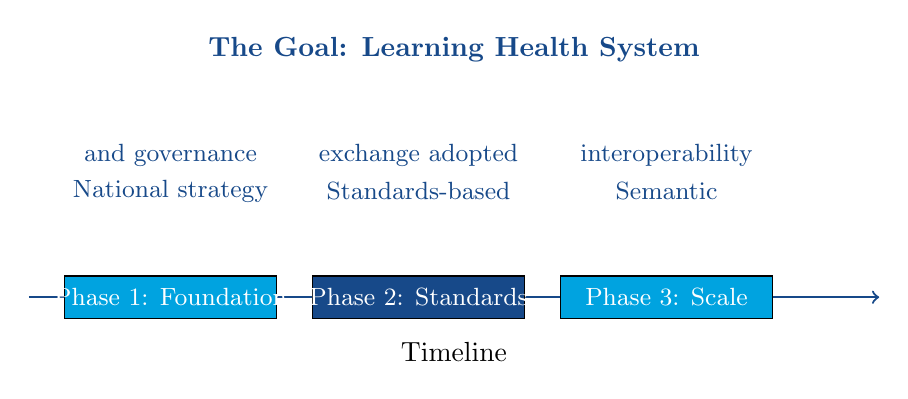
\begin{tikzpicture}[scale=0.9]
            % Roadmap
            \draw[->, thick, darkblue] (0,0) -- (12,0);
            \node[anchor=north] at (6,-0.5) {Timeline};
            
            % Phases
            \draw[fill=accent] (0.5,-0.3) rectangle (3.5,0.3);
            \node[white, font=\small] at (2,0) {Phase 1: Foundation};
            \node[white, font=\small, scale=0.7] at (2,-0.5) {Governance, ID, HIE};
            
            \draw[fill=darkblue] (4,-0.3) rectangle (7,0.3);
            \node[white, font=\small] at (5.5,0) {Phase 2: Standards};
            \node[white, font=\small, scale=0.7] at (5.5,-0.5) {FHIR, Terminology};
            
            \draw[fill=accent] (7.5,-0.3) rectangle (10.5,0.3);
            \node[white, font=\small] at (9,0) {Phase 3: Scale};
            \node[white, font=\small, scale=0.7] at (9,-0.5) {Full integration};
            
            % Key milestones
            \node[darkblue, font=\small] at (2,1.5) {National strategy};
            \node[darkblue, font=\small] at (2,2) {and governance};
            
            \node[darkblue, font=\small] at (5.5,1.5) {Standards-based};
            \node[darkblue, font=\small] at (5.5,2) {exchange adopted};
            
            \node[darkblue, font=\small] at (9,1.5) {Semantic};
            \node[darkblue, font=\small] at (9,2) {interoperability};
            
            % Ultimate goal
            \node[darkblue, font=\bfseries] at (6,3.5) {The Goal: Learning Health System};
        \end{tikzpicture}
    \end{center}
    
    \smallskip
    
    Progress requires phased implementation with clear milestones, sustained commitment, and continuous learning. There is no shortcut to interoperability—only patient, systematic effort across technical, organizational, and policy domains.
\end{frame}

\begin{frame}{Final Reflection}
    \begin{center}
        \begin{quotation}
            \textit{``Interoperability is not merely a technical challenge; it is a social and organizational endeavor that requires alignment of technology, policy, incentives, and culture. The goal—seamless information flow enabling coordinated, safe, effective healthcare—is worth the sustained effort required to achieve it.''}
        \end{quotation}
    \end{center}
    
    \bigskip
    
    Health information interoperability represents one of the most significant opportunities to improve health system performance in the digital age. The challenges are substantial but not insurmountable. Success requires leadership, coordination, and commitment across all stakeholders in the health ecosystem.
    
    \bigskip
    
    \hfill \textbf{Thank you. Questions?}
\end{frame}

%=======================================================================
% REFERENCES
%=======================================================================
\section{References}
\begin{frame}[allowframebreaks]{References}
    \begin{thebibliography}{99}
        
        \bibitem{Abbas2019}
        Abbas, A., et al. (2019). A systematic review of the factors that influence the implementation of health information systems in developing countries. \textit{Journal of Biomedical Informatics}, 94, 103-193.
        
        \bibitem{Adashi2018}
        Adashi, E.Y., \& Cohen, I.G. (2018). To enable the flow of health data: Progress on the 21st Century Cures Act. \textit{JAMA}, 319(16), 1645-1646.
        
        \bibitem{benson2019}
        Benson, T., \& Grieve, G. (2019). \textit{Principles of Health Interoperability: FHIR and HL7}. Cham: Springer Nature.
        
        \bibitem{bloom2019}
        Bloom, S., et al. (2019). Are medical students prepared to participate in health information exchange? \textit{Journal of the American Medical Informatics Association}, 26(12), 1530-1537.
        
        \bibitem{braa2012}
        Braa, J., et al. (2012). Developing health information systems in developing countries: The integrated information system approach. \textit{Mis Quarterly Executive}, 11(2), 73-84.
        
        \bibitem{cohen2018}
        Cohen, I.G., et al. (2018). \textit{Health Data in the Information Age}. New York: NYU School of Law.
        
        \bibitem{EuropeanCommission2021}
        European Commission. (2021). \textit{Proposal for a Regulation on the European Health Data Space}. Brussels: European Commission.
        
        \bibitem{Grannis2019}
        Grannis, S.J., et al. (2019). Evaluating the effect of data standardization and normalization on patient matching quality. \textit{Journal of Biomedical Informatics}, 95, 103-112.
        
        \bibitem{HIMSS2019}
        Healthcare Information and Management Systems Society. (2019). \textit{Interoperability in Healthcare}. Chicago: HIMSS.
        
        \bibitem{IEEE1990}
        Institute of Electrical and Electronics Engineers. (1990). \textit{IEEE Standard Computer Dictionary: A Compilation of IEEE Standard Computer Glossaries}. New York: IEEE.
        
        \bibitem{IHE2020}
        Integrating the Healthcare Enterprise. (2020). \textit{IHE International Annual Report 2020}. Chicago: IHE International.
        
        \bibitem{Jensen2019}
        Jensen, M., et al. (2019). The organizational challenges of cross-border health data exchange: A qualitative study. \textit{BMC Medical Informatics and Decision Making}, 19, 195.
        
        \bibitem{joshi2020}
        Joshi, A., et al. (2020). Ayushman Bharat Digital Mission: Transforming healthcare in India. \textit{Indian Journal of Medical Research}, 152(5), 441-449.
        
        \bibitem{kahn2019}
        Kahn, M.G., et al. (2019). A robust framework for data governance. \textit{AMIA Annual Symposium Proceedings}, 2019, 537-546.
        
        \bibitem{lahyani2019}
        Lahyani, F., et al. (2019). Interoperability in healthcare: Benefits, challenges, and solutions. \textit{International Journal of Medical Informatics}, 124, 31-37.
        
        \bibitem{lehne2019}
        Lehne, M., et al. (2019). Why digital health requires a systems perspective. \textit{Journal of Medical Internet Research}, 21(12), e15049.
        
        \bibitem{McDonald2015}
        McDonald, C.J., et al. (2015). HL7 FHIR: An affordable and interoperable standard for health data exchange. \textit{The Lancet Digital Health}, 1(4), e184-e185.
        
        \bibitem{mendes2019}
        Mendes, R.A., et al. (2019). Digital health in Brazil: Progress and challenges. \textit{Journal of Global Health}, 9(2), 020303.
        
        \bibitem{nyirabagabo2020}
        Nyirabagabo, P., et al. (2020). Building a national health information system in Rwanda: Progress, challenges, and lessons learned. \textit{Global Health: Science and Practice}, 8(3), 467-478.
        
        \bibitem{ODHIN2013}
        ODHIN Consortium. (2013). \textit{Optimizing Delivery of Healthcare Interventions: Framework for Health Information System Strengthening}. Amsterdam: ODHIN.
        
        \bibitem{peterson2019}
        Peterson, K., et al. (2019). A national action plan to achieve health information interoperability in the United States. \textit{Journal of the American Medical Informatics Association}, 26(11), 1322-1332.
        
        \bibitem{richards2018}
        Richards, M., et al. (2018). Mapping between clinical terminologies: Overview and challenges. \textit{Studies in Health Technology and Informatics}, 251, 9-16.
        
        \bibitem{saeed2019}
        Saeed, S., et al. (2019). Building health informatics capacity: An assessment of the current status in low- and middle-income countries. \textit{Journal of Global Health}, 9(2), 020417.
        
        \bibitem{scott2018}
        Scott, P.J., et al. (2018). Frameworks for evaluating national health information systems: A literature review. \textit{Yearbook of Medical Informatics}, 27(1), 94-104.
        
        \bibitem{van Allen2018}
        Van Allen, T.N., et al. (2018). Physician perspectives on long-term patient relationships. \textit{Journal of General Internal Medicine}, 33(8), 1295-1301.
        
        \bibitem{wasunna2020}
        Wasunna, C., et al. (2020). Health information system integration in Kenya: Challenges and opportunities. \textit{East African Medical Journal}, 97(3), 125-134.
        
    \end{thebibliography}
\end{frame}

\end{document}
